\part{ТЕХНОЛОГИЧЕСКИЙ РАЗДЕЛ}

\subsection{Порт RS232}

\subsection{Модули для SRAM-микросхемы M5M5V208FP-85}

Рабочий режим M5M5V208 определяется комбинацией управляющих сигналов устройства $\bar{S_1}$, ${S_2}$, $\bar{W}$ и $\bar{OE}$.\\
Цикл чтения выполняется при низком уровне $\bar{W}$, перекрываемом низким уровнем $\bar{S_1}$ и высоким уровнем ${S_2}$.
Подробнее последовательность действий отражена на Рис.~\ref{ris:sram_write_cycle} и Таблице~\ref{tab:sram_write_cycle}, техническая релизация рассмотрена в
разделе~\ref{sec:sram_controller}. \\

\begin{figure}[H]
\center{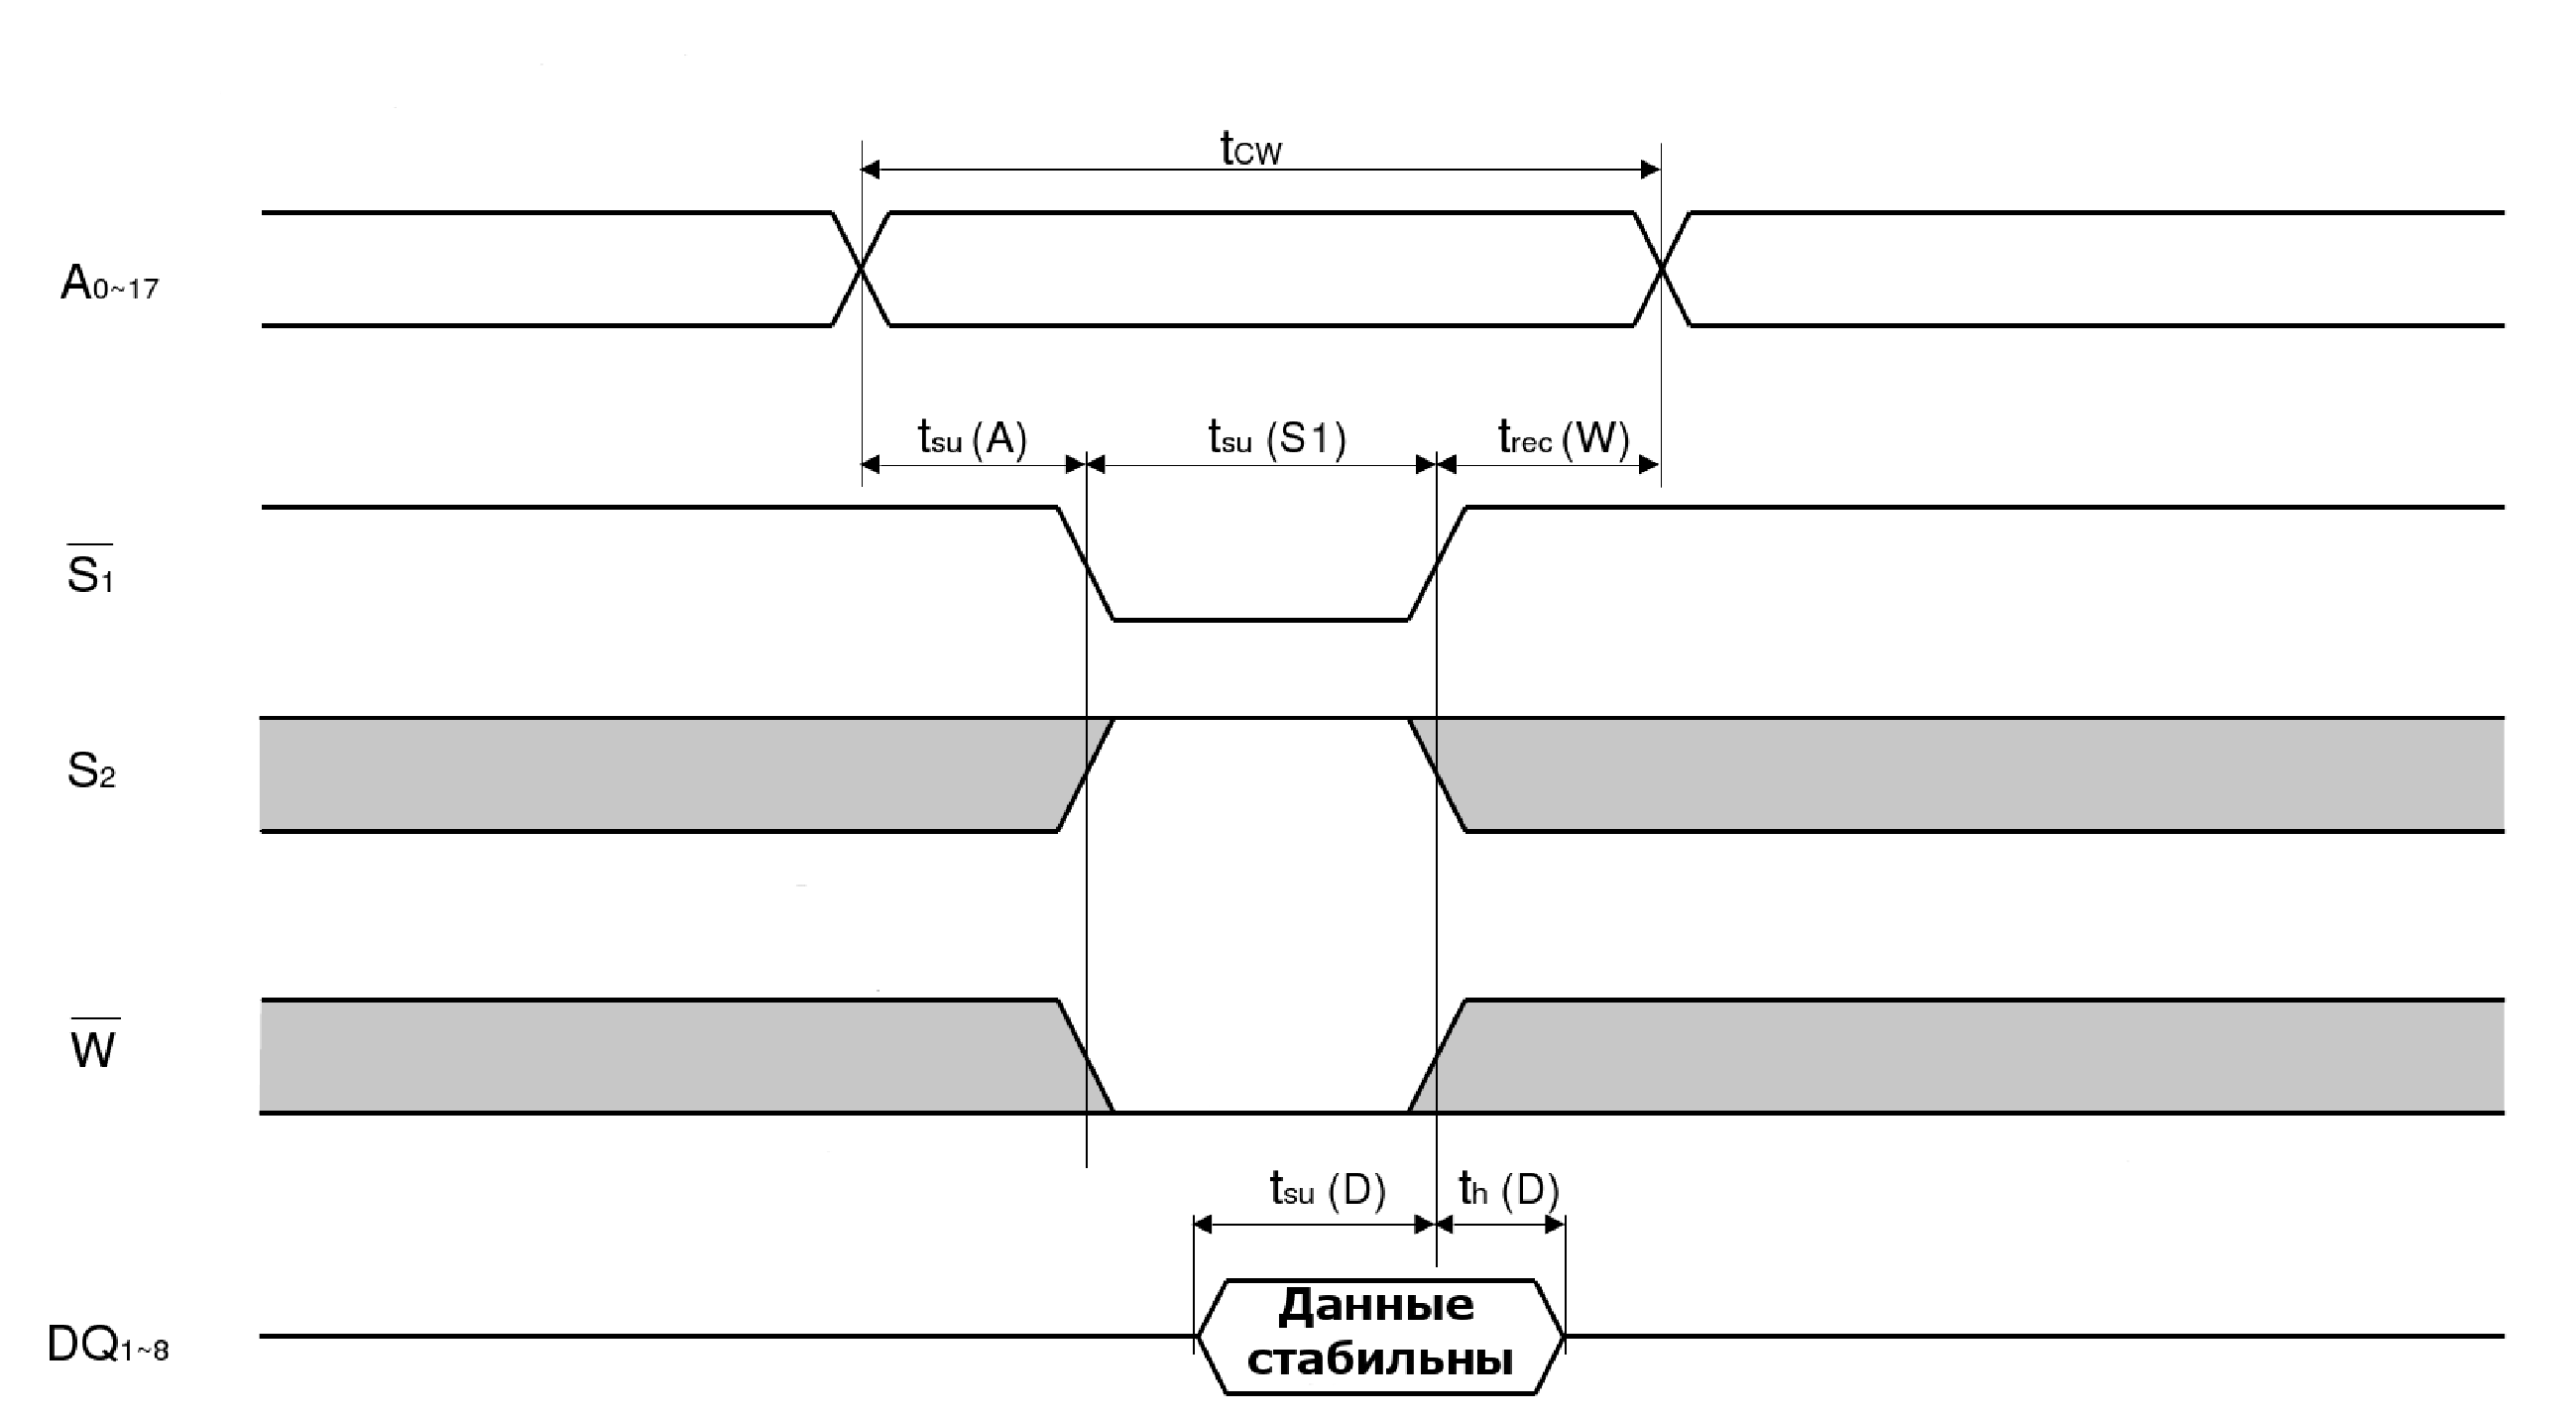
\includegraphics[width=1\linewidth]{./pics/sram_write_cycle.eps} }
\caption{Цикл записи}
\label{ris:sram_write_cycle}
\end{figure}

\begin{table}[H]
\begin{center}
\caption{Цикл операции записи в SRAM}
\label{tab:sram_write_cycle}
\begin{tabular}{|c|c|c|c|}
	\hline
		Название цикла & Обозначение & Время & Единицы \\
	\hline
		${t_{cw}}$ & Время цикла записи & 85 & ns \\
	\hline
		${t_w(W)}$ & Вркмя пульса записи & 60 & ns \\
	\hline
		${t_{su}(A)}$ & Время установки адреса & 0 & ns \\
	\hline
		${t_{su}(A-WH)}$ & Время установки адреса в соотв. с $\bar{E}$ & 70 & ns \\
	\hline
		${t_{su}(S_1)}$ & Время установки Chip Select 1 & 70 & ns \\
	\hline
		${t_{su}(S_2)}$ & Время установки Chip Select 1 & 70 & ns \\
	\hline
		${t_{su}(D)}$ & Время установки данных & 35 & ns \\
	\hline
		${t_{h}(D)}$ & Время удержания данных & 0 & ns \\
	\hline
		${t_{rec}(W)}$ & Время восстановления & 0 & ns \\
	\hline
		${t_{dis}(W)}$ & Время перехода после $\bar{W}$ низкого & 30 & ns \\
	\hline
		${t_{dis}(OE)}$ & Время перехода после $\bar{OE}$ высокого & 30 & ns \\
	\hline
		${t_{en}(W)}$ & Время перехода после $\bar{W}$ высокого & 30 & ns \\
	\hline
		${t_{en}(OE)}$ & Время перехода после $\bar{OE}$ низкого & 30 & ns \\
	\hline
\end{tabular}
\end{center}
\end{table}

Цикл чтения выполняется при высоком уровне сигнала $\bar{W}$ и низком уровне сигнала OE. В то же время сигналы
$\bar{S_1}$ и ${S_2}$ должны находится в активном состоянии. Подробнее последовательность действий отражена на
Рис.~\ref{ris:sram_read_cycle} и Таблице~\ref{tab:sram_read_cycle}.
Техническая реализация рассмотрена в разделе~\ref{sec:sram_controller} \\

\begin{figure}[H]
\center{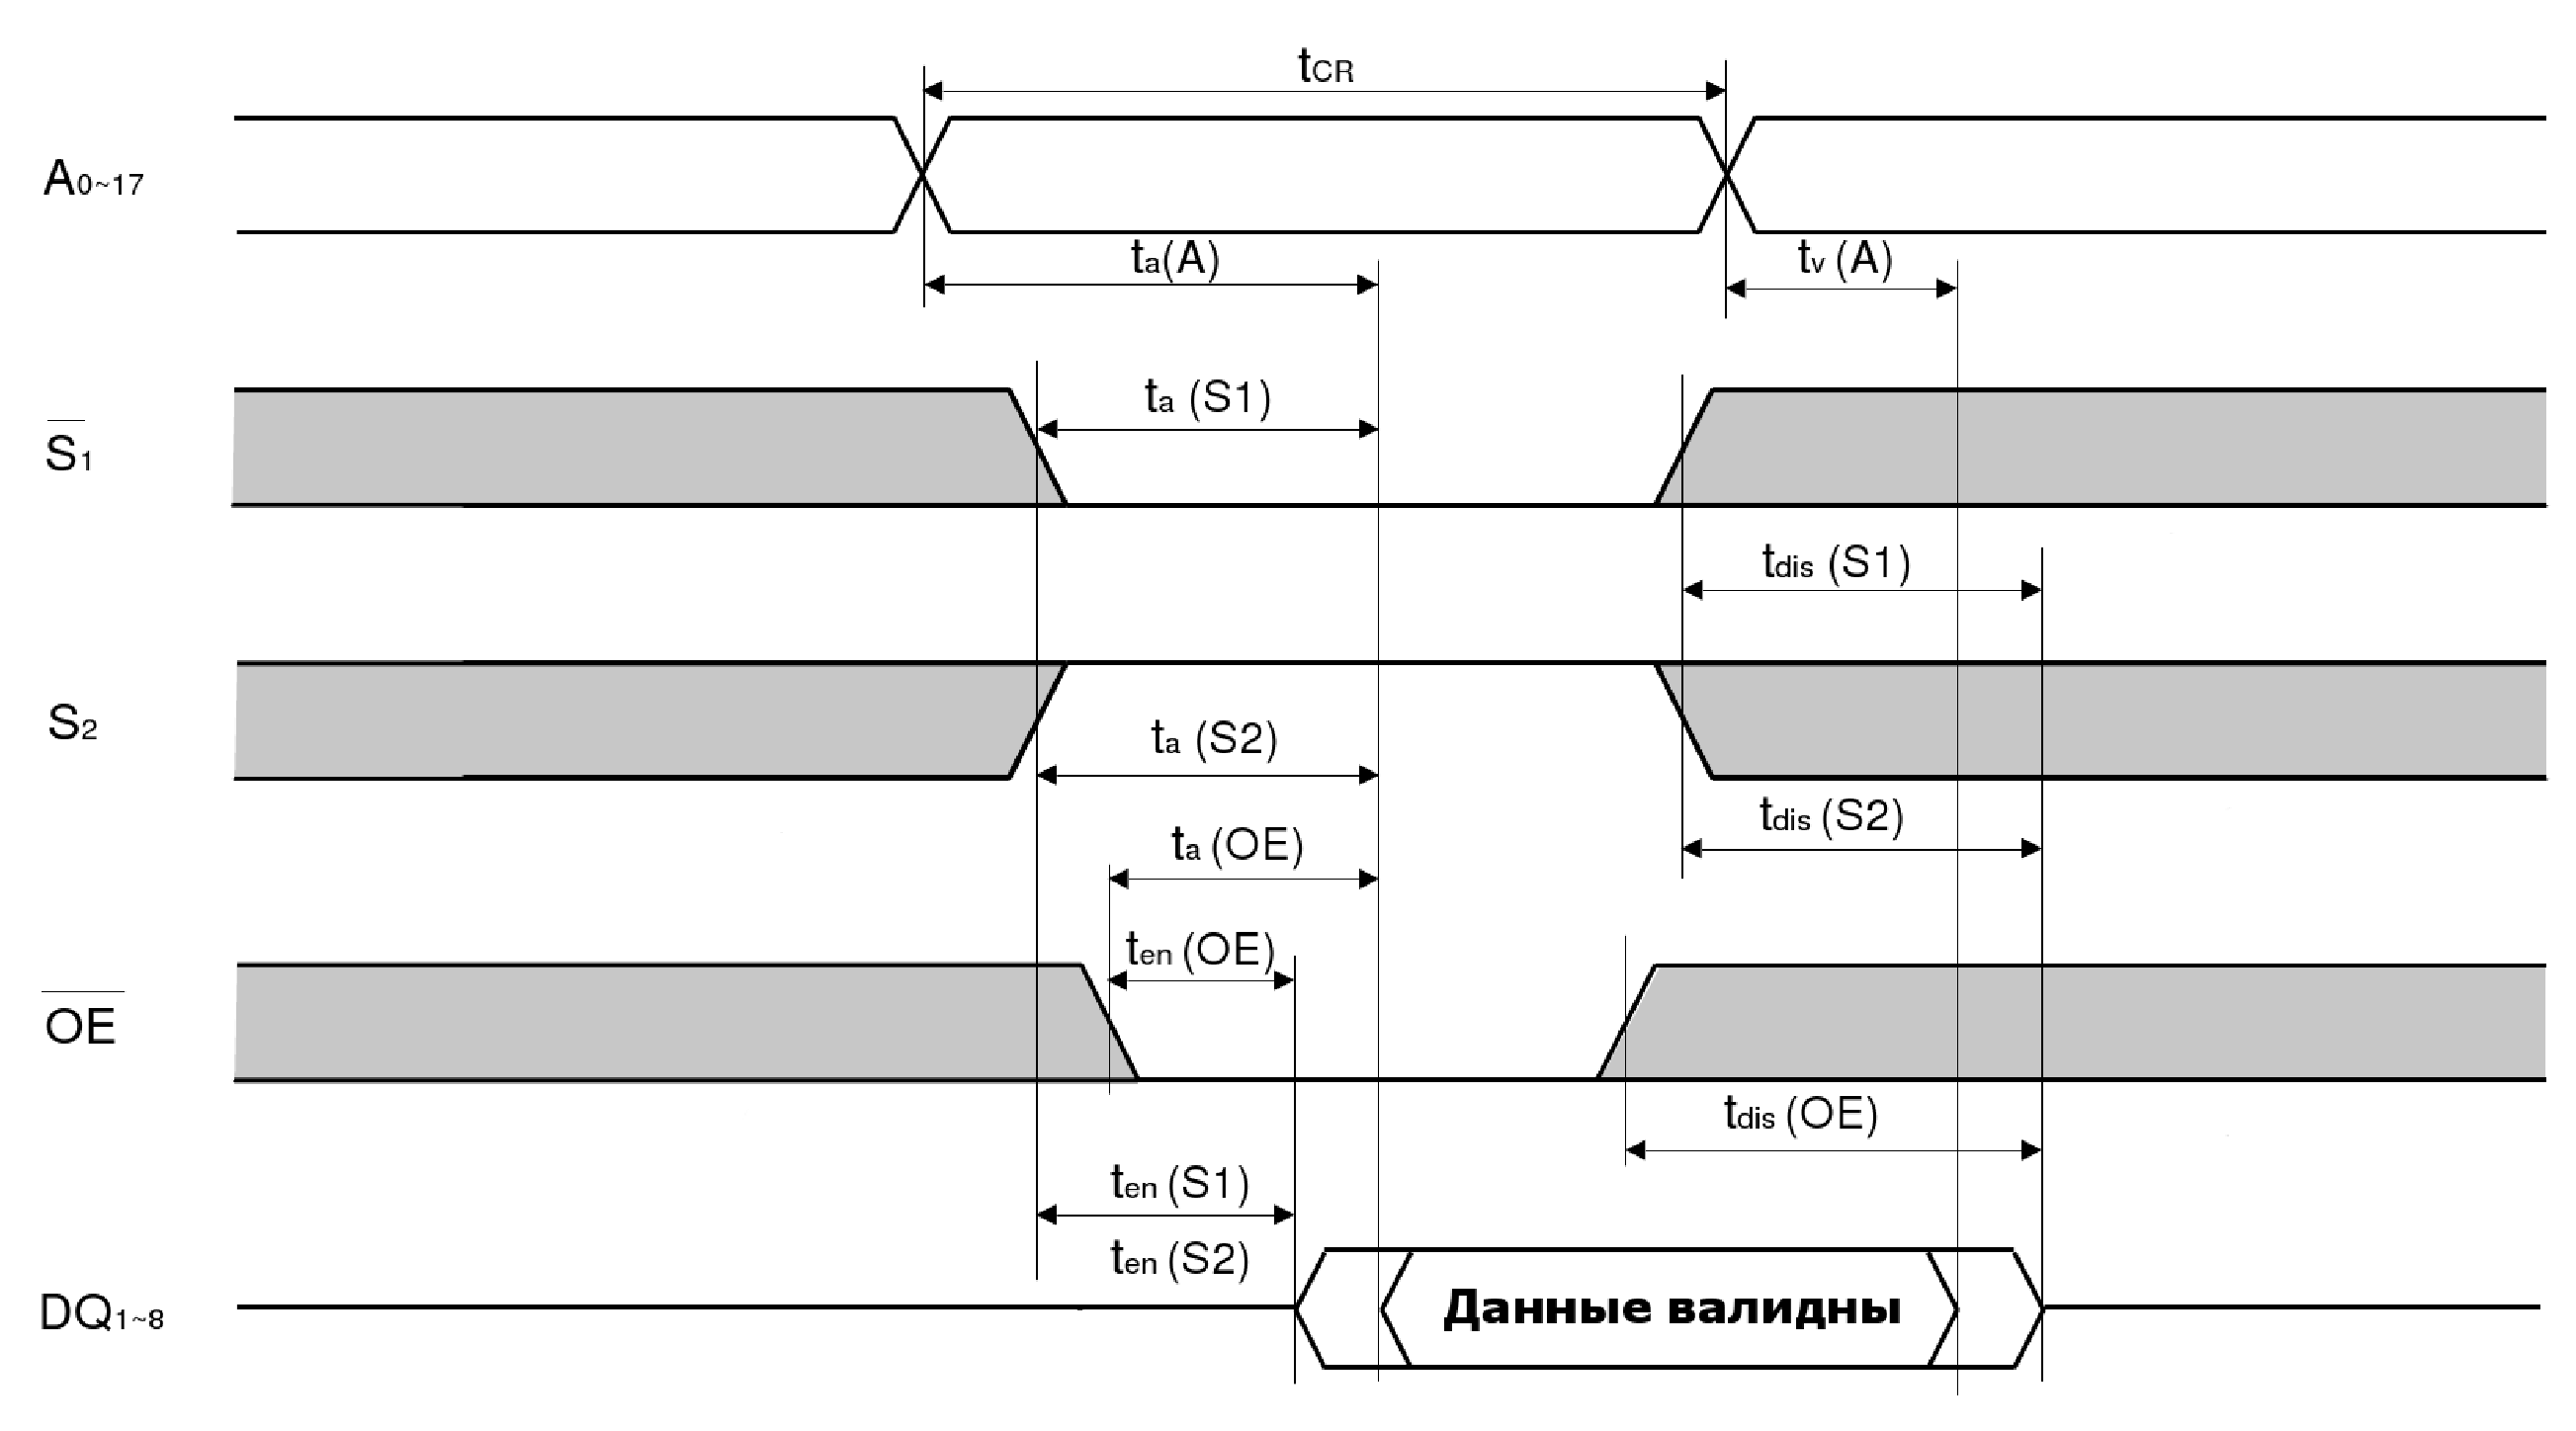
\includegraphics[width=1\linewidth]{./pics/sram_read_cycle.eps}}
\caption{Цикл чтения}
\label{ris:sram_read_cycle}
\end{figure}

\begin{table}[H]
\begin{center}
\caption{Цикл операции чтения из SRAM}
\label{tab:sram_read_cycle}
\begin{tabular}{|c|c|c|c|}
	\hline
		Название цикла & Обозначение & Время & Единицы \\
	\hline
		${t_{cr}(A)}$ & Время цикла чтения & 85 & ns \\
	\hline
		${t_a(A)}$ & Время доступа к адресу & 85 & ns \\
	\hline
		${t_a(S_1)}$ & Chip Select 1 & 85 & ns \\
	\hline
		${t_a(S_1)}$ & Chip Select 2 & 85 & ns \\
	\hline
		${t_a(OE)}$ & Время доступа к активному уровню OE & 45 & ns \\
	\hline
		${t_{dis}(S_1)}$ & Время перехода к низкому уровню & 30 & ns \\
	\hline
		${t_{dis}(S_2)}$ & Время перехода к низкому уровню & 30 & ns \\
	\hline
		${t_{dis}(OE)}$ & Время перехода после $\bar{OE}$ высокого уровня & 30 & ns \\
	\hline
		${t_{en}(S_1)}$ & Переход к активному состоянию для $\bar{S_1}$ & 10 & ns \\
	\hline
		${t_{en}(S_1)}$ & Переход к активному состоянию для ${S_2}$ & 10 & ns \\
	\hline
		${t_{en}(OE)}$ & Переход к активному состоянию для $\bar{OE}$ & 5 & ns \\
	\hline
		${t_{v}(A)}$ & Время валидности данных $\bar{OE}$ & 10 & ns \\
	\hline
\end{tabular}
\end{center}
\end{table}

\newpage

\subsection{Модули для GPS микросхемы MAX2769}

\subsubsection{Serial-интерфейс}
Программирование режимов GPS микросхемы происходит через последовательный порт. Временные критерии и их значения
отражены на Рис.~\ref{ris:gps_serial} и Таблице.~\ref{tab:gps_serial} соответственно. Техническая реализация приведена в
разделе ~\ref{sec:gps_serial}.

\begin{figure}[h]
\center{\includegraphics[width=1\linewidth]{./pics/gps_serial_times.eps}}
\caption{Временная диарамма serial-интерфейса GPS}
\label{ris:gps_serial}
\end{figure}

\begin{table}[h]
\caption{Временные требования для serial-интерфейса}
\label{tab:gps_serial}
\begin{tabular}{|c|p{250pt}|c|p{70pt}|}
 \hline  
  Символ & Параметр & Значение & Единица измерения  \\  
 \hline  
  $t_{css}$  & Время между падающим фронтом сигнала $\bar {CS}$ и передним фронтом сигнала SCLK	& 10 & нс  \\  
 \hline  
  $t_{ds}$   & Время установки данных на serial-линию	& 10 & нс \\  
 \hline  
  $t_{dh}$   & Время удержания данных на serial-линии	& 10 & нс \\  
 \hline  
  $t_{ch}$   & Время нахождения Сlock-сигнала serial-интерфейса в состоянии 1 & 25 & нс \\  
 \hline  
  $t_{cl}$   & Время нахождения Сlock-сигнала serial-интерфейса в состоянии 0 & 25 & нс \\  
 \hline  
  $t_{csh}$  & Время между крайним возрастающим фронтом сигнала SCLK и падающим фронтом сигнала $\bar {CS}$ & 10 & нс \\  
 \hline  
  $t_{csw}$  & Время $\bar {CS}$ в активном состоянии    & 1 & такт \\  
 \hline  
\end{tabular}
\end{table}

%\begin{figure}[h]
%\center{\includegraphics[width=1\linewidth]{./pics/gps_serial_clock_oscylloscope.eps}}
%\caption{Clock-сигнал для serial-интерфейса GPS}
%\end{figure}

\newpage
